\documentclass[conference, onecolumn]{IEEEtran}
\IEEEoverridecommandlockouts
\usepackage{cite}
\usepackage{amsmath,amssymb,amsfonts}
\usepackage{algorithmic}
\usepackage{graphicx}
\usepackage{textcomp}
\usepackage{xcolor}
\usepackage{flushend}
\usepackage{hyperref}
\def\BibTeX{{\rm B\kern-.05em{\sc i\kern-.025em b}\kern-.08em
    T\kern-.1667em\lower.7ex\hbox{E}\kern-.125emX}}
\begin{document}

\title{Final Project Title\\
{\large IOT102-SE18xx, Group x}}

\author{
First Student, Second Student, Third Student, Fourth Student, and Le The Dung\\
FPT University, Ho Chi Minh Campus, Vietnam\\
\{first student, second student, third student, fourth student\}@fpt.edu.vn, dunglt96@fe.edu.vn}
\maketitle

\begin{abstract}
Statement of the purpose of your study the research methods/methodology used to arrive at your results and/or conclusions the results observed the conclusions drawn from your study.
\end{abstract}

\section{Introduction}
Introduce the reason for choosing the topic, briefly present the objectives and content of the topic \cite{Tellez_2016}. \emph{This is an example of a citation.}

\section{Methods and Materials}

\subsection{System Model and Block Diagram}
Draw a block diagram, explain the function of each block and how data is exchanged between blocks.

\begin{figure*}[h]
	\centering
	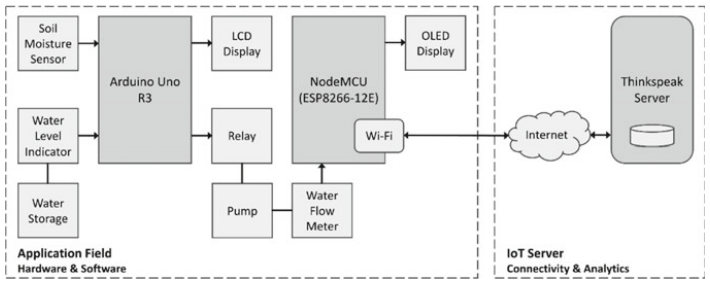
\includegraphics[scale=2]{Block_diagram.png}
	\caption{Block diagram of the developed system.}
	\label{fig}
\end{figure*}

Used \href{https://lucid.app}{https://lucid.app} to draw the block diagram and save it in pdf format.

\subsection{Components and Peripheral Devices}
List all main components used in the developed system. Explain the functions and how to use the components in developed system.

\begin{table}[h]
	\caption{Interfacing between Arduino Uno (or ESP8266) and Its Components}
	\label{tab:my-table}
	\begin{center}
	\begin{tabular}{|l|l|l|l|}
		\hline
		\textbf{Arduino Uno} & \textbf{Soil moisture sensor} & \textbf{LCD display} & \textbf{Relay} \\ \hline
		GND         & GND                  & GND         & GND   \\ \hline
		VCC(5 V)    & VCC                  & VCC         & VCC   \\ \hline
		A0          & A0 (anode)           &             &       \\ \hline
	\end{tabular}
\end{center}
\end{table}

Use \href{https://www.tablesgenerator.com}{https://www.tablesgenerator.com} to create a table online and generate \LaTeX source code for it.

\subsection{Software Programming}
Explain how to set up the IoT platform interface connecting via WiFi/Bluetooth and how to set parameters. Moreover, explain the functionality of the program used for Arduino Uno or NodeMCU ESP8266.

\subsection{Programming Flowchart}
Draw a flowchart and describe the data input and output, data processing process in the developed system.

\section{Results and Discussion}
\subsection{Prototype Implementation}
Describe how to implement the developed system in practice. 

\subsection{Experimental Results}
Include illustrative figures showing the system's operations in different scenarios. Give comments on the results in all figures.

\subsection{Discussion}
Give some discussions about the overall results, the advantages and disadvantages of the developed system.

\section{Conclusion}
Give a clear and concise description of the project’s outputs and the future directions for improving the developed system.

\bibliographystyle{IEEEtran}  %use this for IT
\bibliography{Bib_references}
\end{document}